\documentclass{ximera}
\usepackage{sagetex}
%% handout
%% space
%% newpage
%% numbers
%% nooutcomes

%% You can put user macros here
%% However, you cannot make new environments

\graphicspath{{./}{module1Activity/}{module2Activity/}{module3Activity/}}

\usepackage{sagetex}
\usepackage{tikz}
\usepackage{hyperref}
\usepackage{tkz-euclide}
\usetkzobj{all}
\pgfplotsset{compat=1.7} % prevents compile error.

\tikzstyle geometryDiagrams=[ultra thick,color=blue!50!black]
 %% we can turn off input when making a master document

\outcome{}
\author{Darryl Chamberlain Jr.}
 
\title{Objective 2 - Graph Polynomials}

\begin{document}
\begin{abstract}
Convert between a polynomial function and its graph.
\end{abstract}
\maketitle

\href{https://cnx.org/contents/mwjClAV_@8.1:ZE9qk3Qp@12/Graphs-of-Polynomial-Functions}{Link to section in online textbook.}

%%%%%%%%%%%%%%%%%%%%%
%%%  Objective 2  %%%
%%%%%%%%%%%%%%%%%%%%%

You can print out \href{http://people.clas.ufl.edu/dchamberlain31/files/M6-Objective-2-Graph-Polynomials.pdf}{these notes} to follow along with the video below and keep notes to organize your thoughts.

\youtube{Jv_fdXYq9c4}

Now practice converting between the graph and the corresponding equation. 

\begin{sagesilent}
evenExp1 = ZZ.random_element(2, 5)*2
evenExp2 = ZZ.random_element(2, 5)*2
evenExp3 = ZZ.random_element(2, 5)*2
evenExp4 = ZZ.random_element(2, 5)*2
oddExp1 = ZZ.random_element(2, 5)*2 + 1
oddExp2 = ZZ.random_element(2, 5)*2 + 1
oddExp3 = ZZ.random_element(2, 5)*2 + 1
oddExp4 = ZZ.random_element(2, 5)*2 + 1
\end{sagesilent}

% Q1
\begin{question}
Write an equation of the function graphed below. 

	\begin{center}
	    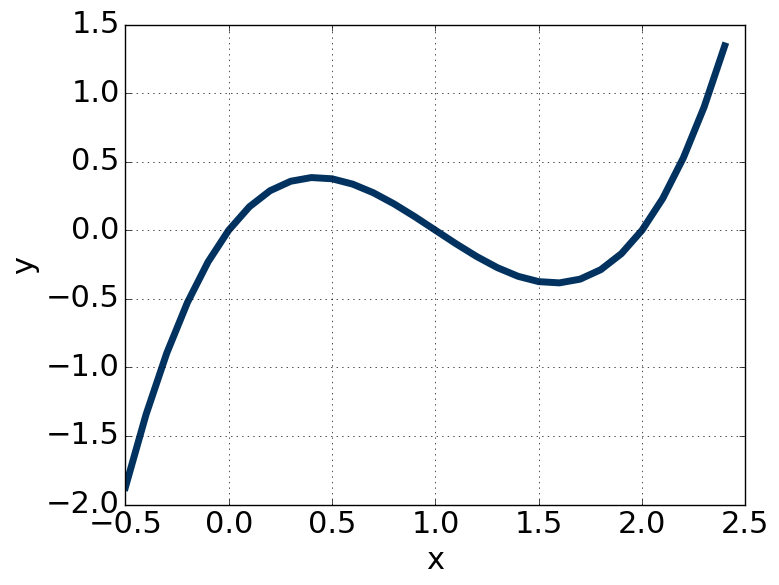
\includegraphics{graphPolyQ1.png}
	\end{center}

\textit{List zeros from smallest to largest. Use $\sage{evenExp1}$ and $\sage{oddExp1}$ as exponents. The leading coefficient is either $1$ or $-1$.}

$f(x) = \answer{1}(x - \answer{0})^{\answer{\sage{oddExp1}}}(x - \answer{1})^{\answer{\sage{oddExp1}}}(x - \answer{2})^{\answer{\sage{oddExp1}}}$
\end{question}

\begin{question}
Write an equation of the function graphed below. 

	\begin{center}
	    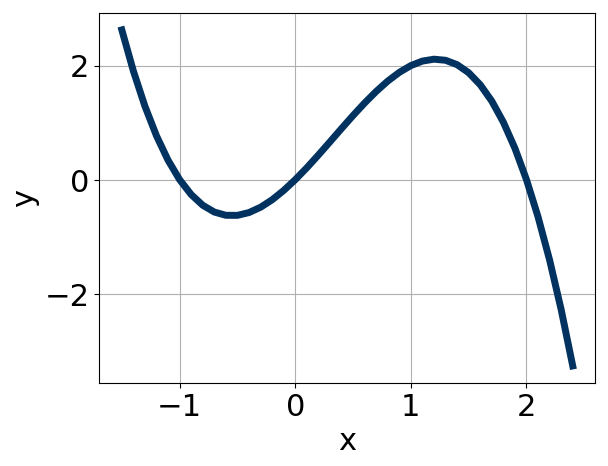
\includegraphics{graphPolyQ2.png}
	\end{center}

\textit{List zeros from smallest to largest. Use $\sage{evenExp2}$ and $\sage{oddExp2}$ as exponents. The leading coefficient is either $1$ or $-1$.}

$f(x) = \answer{-1}(x - \answer{-1})^{\answer{\sage{oddExp2}}}(x - \answer{0})^{\answer{\sage{oddExp2}}}(x - \answer{2})^{\answer{\sage{oddExp2}}}$
\end{question}

% Q3
\begin{question}
Write an equation of the function graphed below. 

	\begin{center}
	    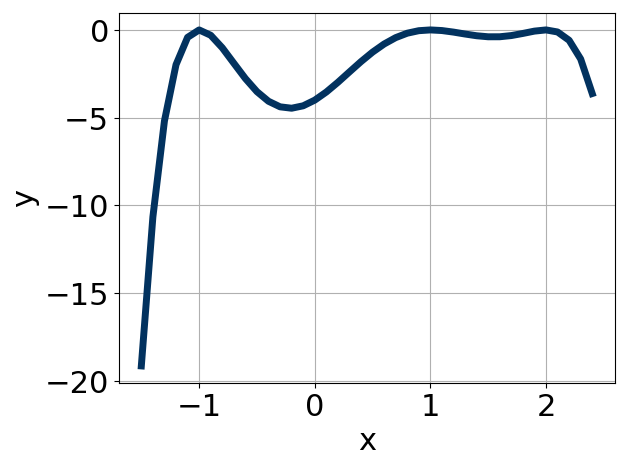
\includegraphics{graphPolyQ3.png}
	\end{center}

\textit{List zeros from smallest to largest. Use $\sage{evenExp3}$ and $\sage{oddExp3}$ as exponents. The leading coefficient is either $1$ or $-1$.}

$f(x) = \answer{-1}(x - \answer{-1})^{\answer{\sage{evenExp3}}}(x - \answer{1})^{\answer{\sage{evenExp3}}}(x - \answer{2})^{\answer{\sage{evenExp3}}}$
\end{question}

\begin{question}
Write an equation of the function graphed below. 

	\begin{center}
	    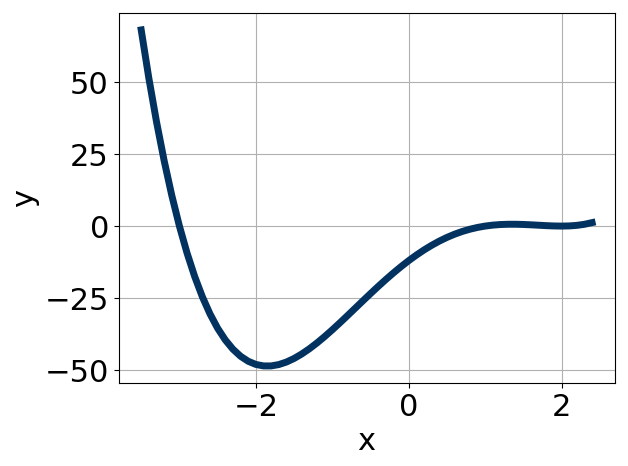
\includegraphics{graphPolyQ4.png}
	\end{center}

\textit{List zeros from smallest to largest. Use $\sage{evenExp4}$ and $\sage{oddExp4}$ as exponents. The leading coefficient is either $1$ or $-1$.}

$f(x) = \answer{1}(x - \answer{-3})^{\answer{\sage{oddExp4}}}(x - \answer{1})^{\answer{\sage{oddExp4}}}(x - \answer{2})^{\answer{\sage{evenExp4}}}$
\end{question}
\end{document}
